\chapter{Negocio}
\section{Introducción}
contenido...
\newpage
%-------------------------------------------------
\section{Punto de Vista de Organización}
El punto de vista de la organización pretende identificar competencias, autoridades y responsabilidades de la organización.
\subsection{Modelo}
\begin{figure}[th!]
	\centering
	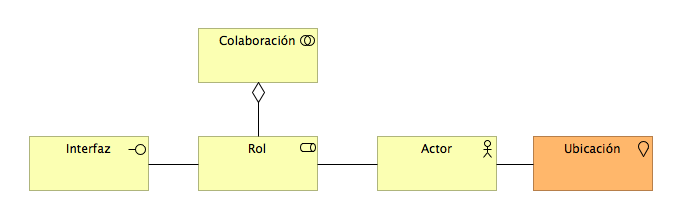
\includegraphics[width=0.8\linewidth]{arquitectura_diseno/imgs/M_Organizacion}
	\caption{Organización}
\end{figure}
\newpage
contenido....
\subsection{Caso}
\begin{figure}[th!]
	\centering
	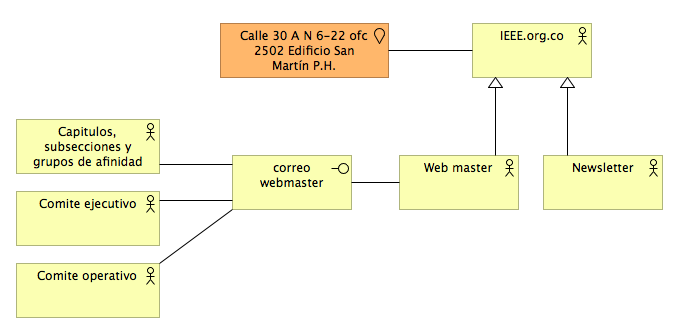
\includegraphics[width=0.8\linewidth]{arquitectura_diseno/imgs/C_Organizacion}
	\caption{Organización}
\end{figure}
%-------------------------------------------------
\newpage
\section{Punto de Vista de Cooperación de Actor}
El punto de vista de la cooperación de actores se centra en las relaciones entre los diferentes actores y su entorno. Permite observar dependencias externas y colaboraciones y muestra la cadena de valor o red en la que opera el actor.
\subsection{Modelo}
\begin{figure}[th!]
	\centering
	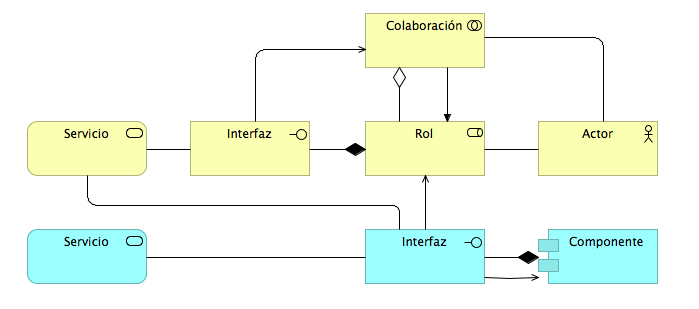
\includegraphics[width=0.8\linewidth]{arquitectura_diseno/imgs/M_Coperacion}
	\caption{Organización}
\end{figure}
\newpage
\subsection{Caso}
\begin{figure}[th!]
	\centering
	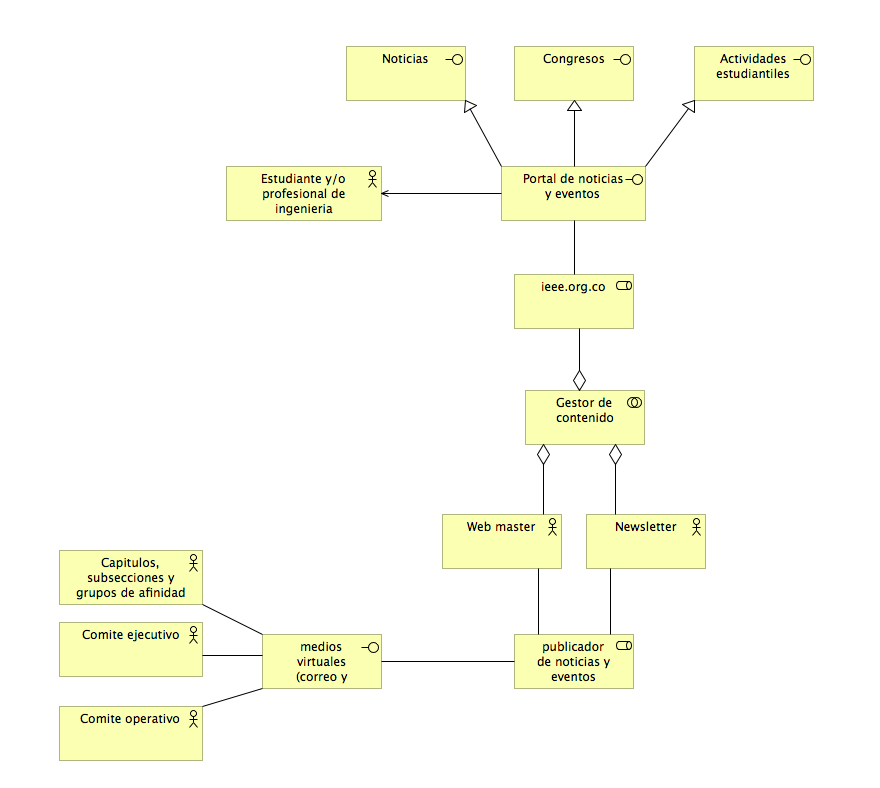
\includegraphics[width=0.8\linewidth]{arquitectura_diseno/imgs/C_Coperacion}
	\caption{Organización}
\end{figure}
%-------------------------------------------------
\newpage
\section{Punto de Vista de Función Negocio}
contenido....
\subsection{Modelo}
\begin{figure}[th!]
	\centering
	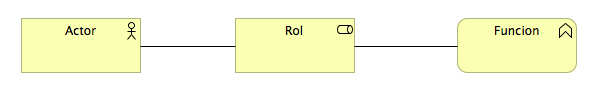
\includegraphics[width=0.8\linewidth]{arquitectura_diseno/imgs/M_FuncionNegocio}
	\caption{Organización}
\end{figure}
\newpage
contenido....
\subsection{Caso}
\begin{figure}[th!]
	\centering
	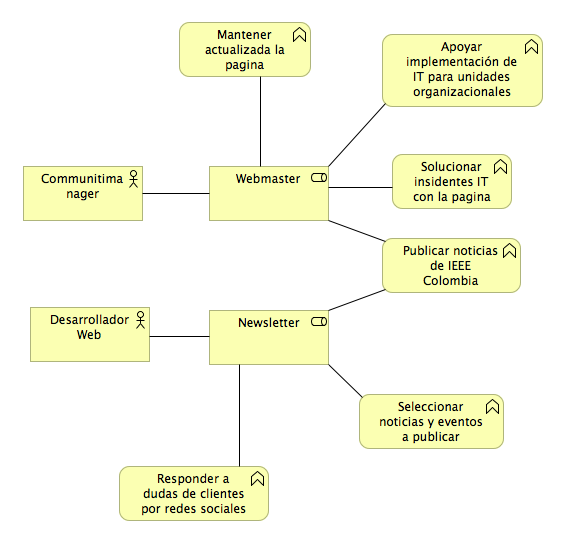
\includegraphics[width=0.8\linewidth]{arquitectura_diseno/imgs/C_Funcion}
	\caption{Organización}
\end{figure}
%-------------------------------------------------
\newpage
\section{Punto de Vista de Proceso}
contenido....
\subsection{Modelo}
\begin{figure}[th!]
	\centering
	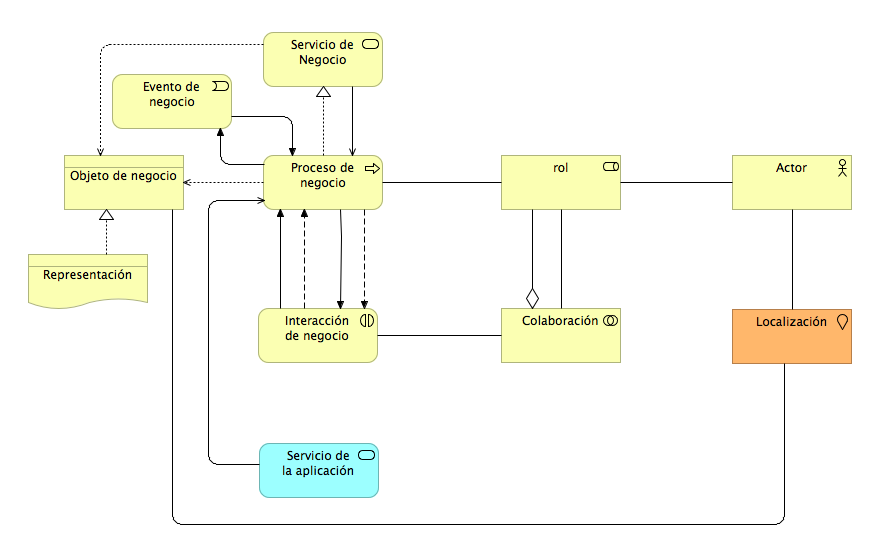
\includegraphics[width=0.8\linewidth]{arquitectura_diseno/imgs/M_ProcesoNegocio}
	\caption{Organización}
\end{figure}
\newpage
contenido....
\subsection{Caso}
\begin{figure}[th!]
	\centering
	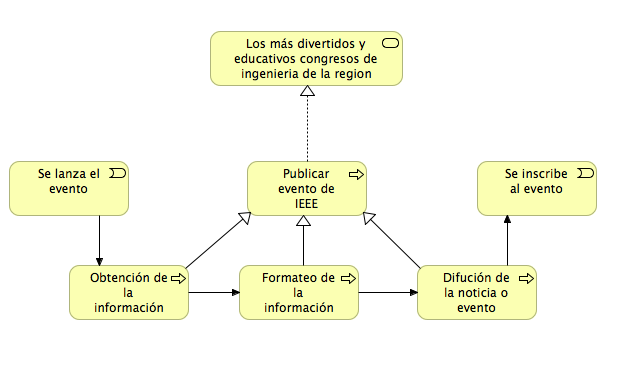
\includegraphics[width=0.8\linewidth]{arquitectura_diseno/imgs/C_ProcesoNegocio}
	\caption{Organización}
\end{figure}
%-------------------------------------------------
\newpage
\section{Punto de Vista de Cooperación de Proceso}
contenido....
\subsection{Modelo}
\begin{figure}[th!]
	\centering
	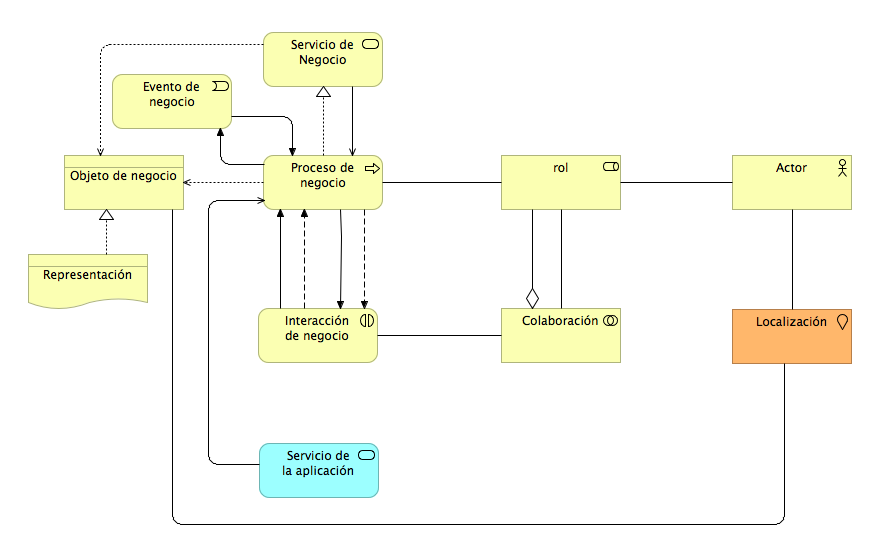
\includegraphics[width=0.8\linewidth]{arquitectura_diseno/imgs/M_CoperacionProceso}
	\caption{Organización}
\end{figure}
\newpage
contenido....
\subsection{Caso}
\begin{figure}[th!]
	\centering
	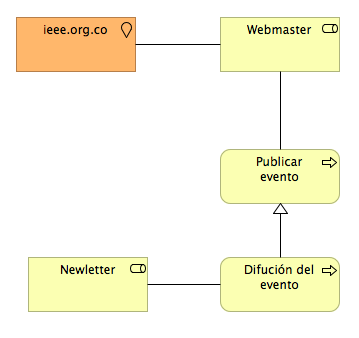
\includegraphics[width=0.8\linewidth]{arquitectura_diseno/imgs/C_CoperacionProceso}
	\caption{Organización}
\end{figure}
%-------------------------------------------------
\newpage
\section{Punto de Vista de Producto}
contenido....
\subsection{Modelo}
\begin{figure}[th!]
	\centering
	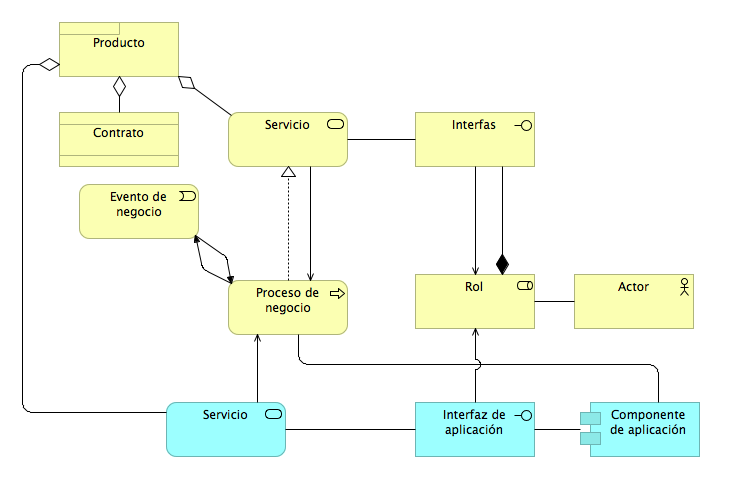
\includegraphics[width=0.8\linewidth]{arquitectura_diseno/imgs/M_Producto}
	\caption{Organización}
\end{figure}
\newpage
contenido....
\subsection{Caso}
\begin{figure}[th!]
	\centering
	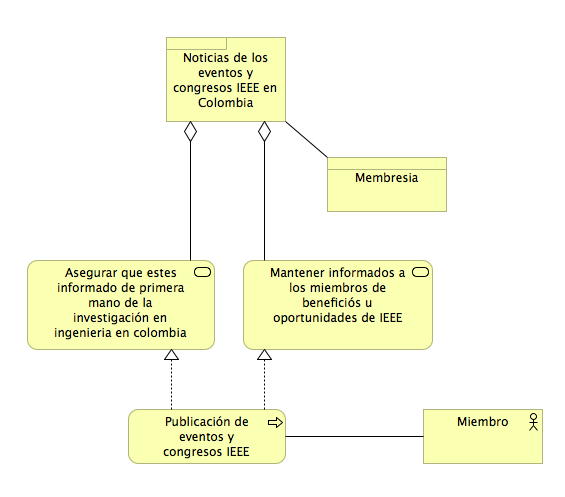
\includegraphics[width=0.8\linewidth]{arquitectura_diseno/imgs/C_Producto}
	\caption{Organización}
\end{figure}